% Generated with genpdf
% Domain Interno
% Title Piano di Progetto
\documentclass{scalatekids-article}
\begin{document}
\lfoot{Piano Di Progetto 0.1.0}
\begin{titlepage}
  \centering
  
\includegraphics[width=0.45\textwidth]{logo.png}\par\vspace{1cm}
  \vspace{1.5cm}
         {\Huge\bfseries Piano Di Progetto \par}
         \begin{center}
           \vspace{1.0cm}
                  {\large\bfseries Informazioni sul documento \par}
         \end{center}
         \vspace{-1cm}
         \begin{center}
           \line(1,0){300}
         \end{center}
         \vspace{0cm}
         \begin{tabular}[c]{l|l}
           \textbf{Versione} & 0.1.0\\
           \textbf{Redazione} & Redattore1\\ & Redattore2\\ & Redattore3..\\
           \textbf{Verifica} & Verificatore1\\ & Verificatore2..\\
           \textbf{Responsabile} & Responsabile\\
           \textbf{Uso} & Esterno\\
           \textbf{Lista di distribuzione} & ScalateKids
         \end{tabular}
\end{titlepage}
\clearpage
\setcounter{page}{1}
\begin{flushleft}
  \vspace{0cm}
         {\large\bfseries Diario delle modifiche \par}
\end{flushleft}
\vspace{0cm}
\begin{center}
  \begin{tabular}{| l | l | l | l | l |}
    \hline
    Versione & Autore & Ruolo & Data & Descrizione \\
    \hline
    0.1.1 & Andrea Giacomo Baldan & Responsabile & 2015-12-28 & Stesura pianificazione preventiva\\
    \hline
    0.1.0 & Andrea Giacomo Baldan & Responsabile & 2015-12-23 & Stesura analisi dei rischi \\
    \hline
    0.0.6 & Marco Boseggia & Analista & 2015-12-23 & Redazione scelta del modello di ciclo di vita\\
    \hline
    0.0.5 & Marco Boseggia & Analista & 2015-12-22 & Stesura Organigramma\\
    \hline
    0.0.1 & Andrea Giacomo Baldan & Responsabile & 2015-12-21 & Creazione scheletro del documento\\
    \hline
  \end{tabular}
\end{center}
\tableofcontents
\newpage
\section{Sommario}
\subsection{Scopo del documento}
Il seguente documento ha lo scopo di specificare il piano con cui il gruppo \textit{ScalateKids} lavorerà sul progetto \textbf{Actorbase}.
Nel documento verranno specificati:
\begin{itemize}
\item {L'\gloss{organigramma} del gruppo;}
\item {L'analisi preventiva dell'utilizzo delle risorse;}
\item {L'utilizzo delle risorse durante lo svolgersi del progetto;}
\item {L'analisi dei fattori di rischio.}
\end{itemize}
\prodPurpose
\glossExpl
\subsection{Scelta del modello di ciclo di vita}
Per lo sviluppo del progetto \textbf{Actorbase} il gruppo ha scelto di applicare ai processi il modello incrementale. Questa scelta è dovuta alle seguenti proprietà offerte da questo modello:
\begin{itemize}
\item {La scomposizione del sistema in sottosistemi di dimensione minore;}
\item {I cicli di incrementi pianificati;}
\item {Il rilascio di più \gloss{prototipi} durante lo sviluppo.}
\end{itemize}
La scomposizione in sottosistemi comporta la possibilità di concentrare le risorse su un numero limitato di attività semplificando la gestione delle risorse e del tempo. Inoltre è possibile scegliere le attività su cui concentrarsi in modo da soddisfare per primi i requisiti più critici. In questo modo i componenti che soddisfano i requisiti principali vengono testati più volte e raffinati maggiormente rispetto ai requisiti opzionali. Questa suddivisione aiuta anche la fase di verifica e test, in quanto rende possibile il test su componenti piccole, rendendo i test più precisi. Le attività di analisi e progettazione dell'architettura ad alto livello vengono svolti una volta sola, dopo aver fissato i requisiti principali è possibile definire l'architettura del sistema. Questo modello consente di avere un prototipo con delle funzionalità di primaria importanza durante la fase di sviluppo, così da poter avere un confronto con il Committente in corso d'opera. A partire da questa base ogni incremento aggiunge nuove funzionalità al prodotto garantendo quindi una convergenza entro tempi e costi preventivati.
\subsection{Scadenze}
Le attività di pianificazione del progetto saranno basate sulle scadenze qui riportate:
\begin{itemize}
\item {Revisione dei Requisiti (RR): 2016-01-22;}
\item {Revisione di Progetto (RP): ;}
\item {Revisione di Qualifica (RQ): ;}
\item {Revisione di Accettazione (RA): .}
\end{itemize}
\section{Organigramma}
\subsection{Accettazione componenti}
\begin{center}
  \begin{tabular}{|l | l | p{4cm} |}
    \hline
    Nome & Data & Firme \\
    \hline
    Alberto De Agostini & 2015-12-18 &\\
    Andrea Giacomo Baldan & 2015-12-18 &\\
    Marco Boseggia & 2015-12-18 &\\
    Giacomo Vanin & 2015-12-18 &\\
    Michael Munaro & 2015-12-18 &\\
    Davide Trevisan & 2015-12-18 &\\
    Francesco Agostini & 2015-12-18 &\\
    \hline
  \end{tabular}
\end{center}
\subsection{Componenti}
\begin{center}
  \begin{tabular}{|l | l | l |}
    \hline
    Nome & Matricola & Email \\
    \hline
    Alberto De Agostini & 579021 & albertodeagostini88@gmail.com\\
    Andrea Giacomo Baldan & 579117 & a.g.baldan@gmail.com\\
    Marco Boseggia & 1044608 & boseggiam91@gmail.com\\
    Giacomo Vanin & 1026988 & giacomo.vanin92@gmail.com\\
    Michael Munaro & 1049522 & munaro.michael@gmail.com\\
    Davide Trevisan & 1070686 & trevisan.davide94@libero.it\\
    Francesco Agostini & 1051519 & francesco.agostini.93@gmail.com\\
    \hline
  \end{tabular}
\end{center}
\section{Pianificazione preventiva}
\subsection{Suddivisione fasi}
\label{sub:fasi}
Per semplificare la pianificazione del prospetto orario, sono state identificate
tre fasi principali che rappresentano l'intero ciclo di sviluppo del prodotto.\\
% TODO: da proseguire
Esse sono:
\begin{itemize}
\item\textbf{Analisi:} Rappresenta la prima fase del progetto, dalla
  pubblicazione dei capitolati d'appalto all'inizio della fase di progettazione,
  comprensiva di una fase di incremento, ove vengono risolti i possibili dubbi
  emersi in prima stesura.\\
  Figure maggiormente coinvolte: \textit{Responsabile, Amministratore, Analista, Verificatore}
\item\textbf{Progettazione:} Segue la fase di Analisi, e racchiude il lasso
  temporale dedicato alla correzione degli errori rilevati in sede di Revisione di Requisiti e alla progettazione dell'architettura sulla base dei requisiti
  emersi. Comprende anche lo studio di \gloss{design pattern} congrui alla realizzazione
  del prodotto.\\
  Figure maggiormente coinvolte: \textit{Responsabile, Amministratore, Progettista, Verificatore}
\item\textbf{Codifica:} L'ultima delle tre fasi identificate, comprende la correzione degli errori rilevati in sede di Revisione di Progettazione e la stesura
  del codice secondo le direttive emerse in fase di progettazione.\\
  Figure maggiormente coinvolte: \textit{Responsabile, Amministratore, Programmatore, Verificatore}
\end{itemize}
Tutte e tre le fasi descritte sono comprensive di \textbf{Verifica e
  validazione}, assimilabile ad una fase ``fittizzia'', in quanto è
presente lungo tutto l'arco di sviluppo del prodotto.\\
Ogni fase prevede l'impiego di alcuni ruoli in misura maggiore rispetto ad
altri, nella distribuzione di questi sarà garantita un equa ripartizione del
carico di lavoro individuale.\\
Come riportato nelle \href{run:../Interni/NormeDiProgetto\_v0.0.1.pdf}{Norme Di Progetto v0.0.1}
ogni componente del gruppo potrà ricoprire più ruoli contemporaneamente, purchè sia
garantita l'assenza di conflitti d'interesse tra le attività svolte.
\newpage
\subsubsection{Analisi}
Nella fase di Analisi, i componenti ricopriranno i ruoli di progetto secondo la distribuzione seguente:
\begin{center}
  \scriptsize
  \begin{tabular}{| c | p{0.35cm} p{0.35cm} | p{0.35cm} p{0.35cm} | p{0.35cm} p{0.35cm} | p{0.35cm} p{0.35cm} | p{0.35cm} p{0.35cm} | p{0.35cm} p{0.35cm} | p{0.35cm} p{0.35cm} |}
    \hline
    \textbf{Nome} & \multicolumn{2}{|c|}{\textbf{Res}} & \multicolumn{2}{|c|}{\textbf{An}} & \multicolumn{2}{|c|}{\textbf{Amm}} & \multicolumn{2}{|c|}{\textbf{Pr}} & \multicolumn{2}{|c|}{\textbf{Pt}} & \multicolumn{2}{|c|}{\textbf{Ve}} & \multicolumn{2}{|c|}{\textbf{Tot}}\\
    \hline
    & \textbf{Inv} & \textbf{Ren} & \textbf{Inv} & \textbf{Ren} & \textbf{Inv} & \textbf{Ren} & \textbf{Inv} & \textbf{Ren} & \textbf{Inv} & \textbf{Ren} & \textbf{Inv} & \textbf{Ren} & \textbf{Inv} & \textbf{Ren}\\
    \hline
    Andrea Baldan & 13 & 12 & & & 10 & 7 & & & & & 12 & 10 & 35 & 29\\
    Alberto de Agostini & 12 & 11 & 12 & 10 & & & & & & & 12 & 9 & 36 & 30\\
    Michael Munaro & & & 17 & 15 & & & & & & & 17 & 14 & 34 & 29\\
    Giacomo Vanin & & & 17 & 14 & & & & & & & 19 & 17 & 36 & 31\\
    Marco Boseggia & & & 18 & 16 & & & & & & & 16 & 15 & 34 & 31\\
    Francesco Agostini & & & 10 & 9 & 10 & 8 & & & & & 14 & 12 & 34 & 29\\
    Davide Trevisan & & & 14 & 12 & & & & & & & 13 & 11 & 27 & 23\\
    \hline
  \end{tabular}
\end{center}
I seguenti grafici illustrano le ore investite per Persona suddivise tra ore investite e ore rendicontate, in fase di Analisi
\begin{figure}[H]
  \begin{subfigure}[H]{0.47\textwidth}
    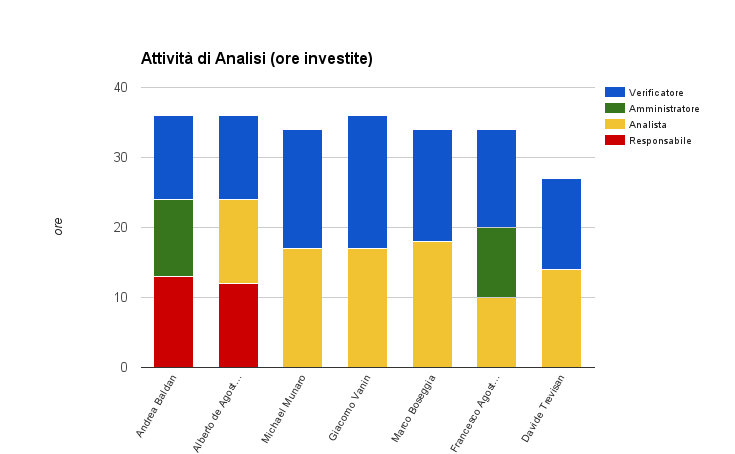
\includegraphics[width=1.2\textwidth,keepaspectratio]{AnalisiConInvestimento.png}
    \caption{Ore con investimento, fase di Analisi}
  \end{subfigure}
  \qquad
  \begin{subfigure}[H]{0.47\textwidth}
    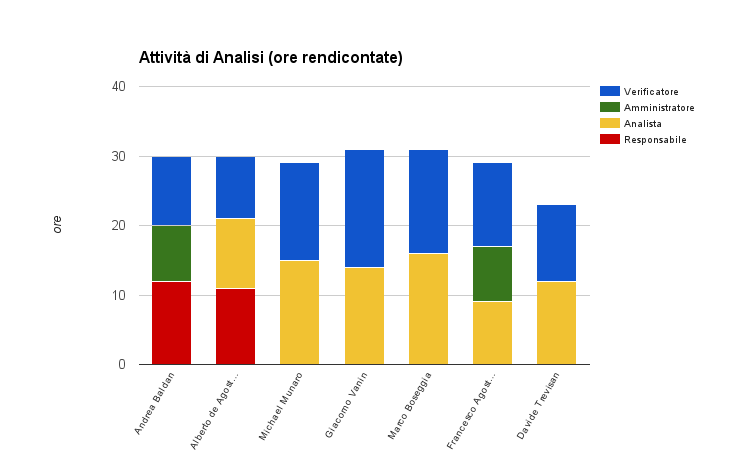
\includegraphics[width=1.2\textwidth,keepaspectratio]{AnalisiConRendicontazione.png}
    \caption{Ore con rendicontazione, fase di Analisi}
  \end{subfigure}
\end{figure}

\newpage
\subsubsection{Progettazione}
Nella fase di Progettazione, i componenti ricopriranno i ruoli di progetto secondo la distribuzione seguente:
\begin{center}
  \scriptsize
  \begin{tabular}{| c | p{0.35cm}  p{0.35cm} | p{0.35cm}  p{0.35cm} | p{0.35cm}  p{0.35cm} | p{0.35cm}  p{0.35cm} | p{0.35cm}  p{0.35cm} | p{0.35cm}  p{0.35cm} | p{0.35cm}  p{0.35cm} |}
    \hline
    \textbf{Nome} & \multicolumn{2}{|c|}{\textbf{Res}} & \multicolumn{2}{|c|}{\textbf{An}} & \multicolumn{2}{|c|}{\textbf{Amm}} & \multicolumn{2}{|c|}{\textbf{Pr}} & \multicolumn{2}{|c|}{\textbf{Pt}} & \multicolumn{2}{|c|}{\textbf{Ve}} & \multicolumn{2}{|c|}{\textbf{Tot}}\\
    \hline
    & \textbf{Inv} & \textbf{Ren} & \textbf{Inv} & \textbf{Ren} & \textbf{Inv} & \textbf{Ren} & \textbf{Inv} & \textbf{Ren} & \textbf{Inv} & \textbf{Ren} & \textbf{Inv} & \textbf{Ren} & \textbf{Inv} & \textbf{Ren}\\
    \hline
    Andrea Baldan & & & & & & & 17 & 14 & & & 12 & 11 & 29 & 25\\
    Alberto de Agostini & & & 5 & 4 & 4 & 4 & 20 & 18 & & & & & 29 & 26\\
    Michael Munaro & & & & & 6 & 5 & & & & & 19 & 17 & 25 & 22\\
    Giacomo Vanin & 11 & 10 & & & & & 18 & 16 & & & & & 29 & 26\\
    Marco Boseggia & 10 & 8 & 7 & 6 & & & 4 & 3 & & & 18 & 15 & 39 & 32\\
    Francesco Agostini & & & 8 & 7 & & & 17 & 15 & & & & & 25 & 22\\
    Davide Trevisan & & & 8 & 6 & & & 18 & 16 & & & 15 & 12 & 41 & 34\\
    \hline
  \end{tabular}
\end{center}
I seguenti grafici illustrano le ore investite per Persona suddivise tra ore investite e ore rendicontate, in fase di Progettazione
\begin{figure}[H]
  \begin{subfigure}[H]{0.47\textwidth}
    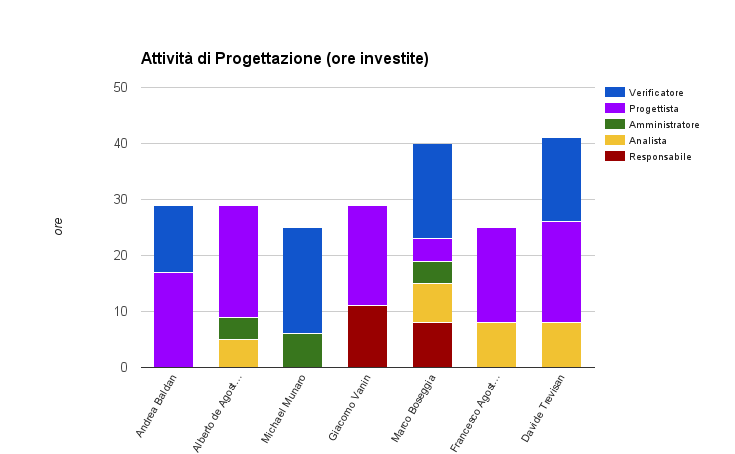
\includegraphics[width=1.2\textwidth,keepaspectratio]{ProgettazioneConInvestimento.png}
    \caption{Ore con investimento, fase di Progettazione}
  \end{subfigure}
  \qquad
  \begin{subfigure}[H]{0.47\textwidth}
    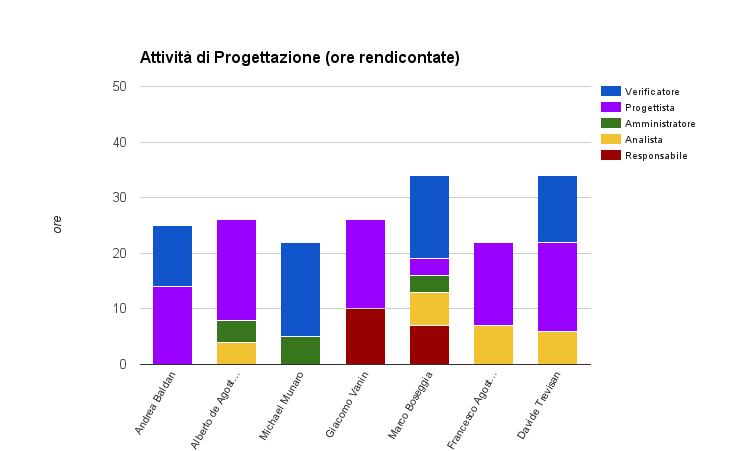
\includegraphics[width=1.2\textwidth,keepaspectratio]{ProgettazioneConRendicontazione.png}
    \caption{Ore con rendicontazione, fase di Progettazione}
  \end{subfigure}
\end{figure}
\newpage
\subsubsection{Codifica}
Nella fase di Codifica, i componenti ricopriranno i ruoli di progetto secondo la distribuzione seguente:
\begin{center}
  \scriptsize
  \begin{tabular}{| c | p{0.35cm}  p{0.35cm} | p{0.35cm}  p{0.35cm} | p{0.35cm}  p{0.35cm} | p{0.35cm}  p{0.35cm} | p{0.35cm}  p{0.35cm} | p{0.35cm}  p{0.35cm} | p{0.35cm}  p{0.35cm} |}
    \hline
    \textbf{Nome} & \multicolumn{2}{|c|}{\textbf{Res}} & \multicolumn{2}{|c|}{\textbf{An}} & \multicolumn{2}{|c|}{\textbf{Amm}} & \multicolumn{2}{|c|}{\textbf{Pr}} & \multicolumn{2}{|c|}{\textbf{Pt}} & \multicolumn{2}{|c|}{\textbf{Ve}} & \multicolumn{2}{|c|}{\textbf{Tot}}\\
    \hline
    & \textbf{Inv} & \textbf{Ren} & \textbf{Inv} & \textbf{Ren} & \textbf{Inv} & \textbf{Ren} & \textbf{Inv} & \textbf{Ren} & \textbf{Inv} & \textbf{Ren} & \textbf{Inv} & \textbf{Ren} & \textbf{Inv} & \textbf{Ren}\\
    \hline
    Andrea Baldan & & & 2 & 2 & & & 22 & 20 & 26 & 24 & 2 & 2 & 52 & 48\\
    Alberto de Agostini & & & & & & & 21 & 18 & 17 & 15 & 16 & 12 & 54 & 45\\
    Michael Munaro & 10 & 9 & & & & & & & 31 & 27 & 22 & 17 & 63 & 53\\
    Giacomo Vanin & & & & & 6 & 5 & & & 24 & 21 & 24 & 18 & 54 & 44\\
    Marco Boseggia & & & & & & & 23 & 20 & 22 & 20 & & & 45 & 40\\
    Francesco Agostini & 8 & 7 & & & & & 27 & 24 & & & 25 & 20 & 60 & 51\\
    Davide Trevisan & 6 & 6 & & & & & 24 & 22 & 10 & 9 & 13 & 9 & 53 & 46\\
    \hline
  \end{tabular}
\end{center}
\normalsize
I seguenti grafici illustrano le ore investite per Persona suddivise tra ore investite e ore rendicontate, in fase di Codifica
\begin{figure}[H]
  \begin{subfigure}[H]{0.47\textwidth}
    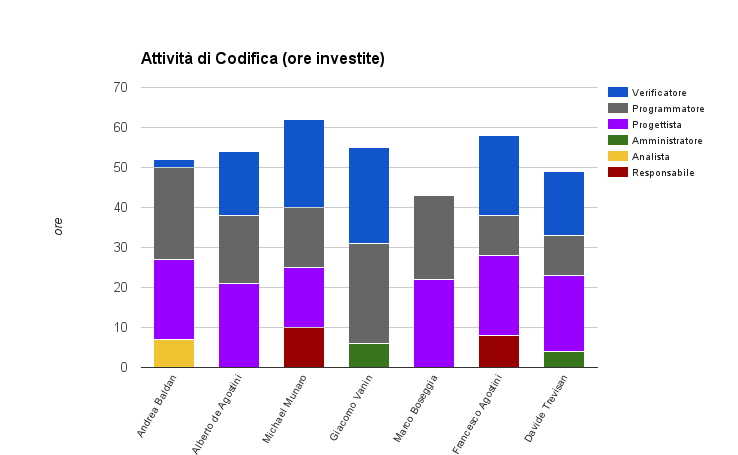
\includegraphics[width=1.2\textwidth,keepaspectratio]{CodificaConInvestimento.png}
    \caption{Ore con investimento, fase di Codifica}
  \end{subfigure}
  \qquad
  \begin{subfigure}[H]{0.47\textwidth}
    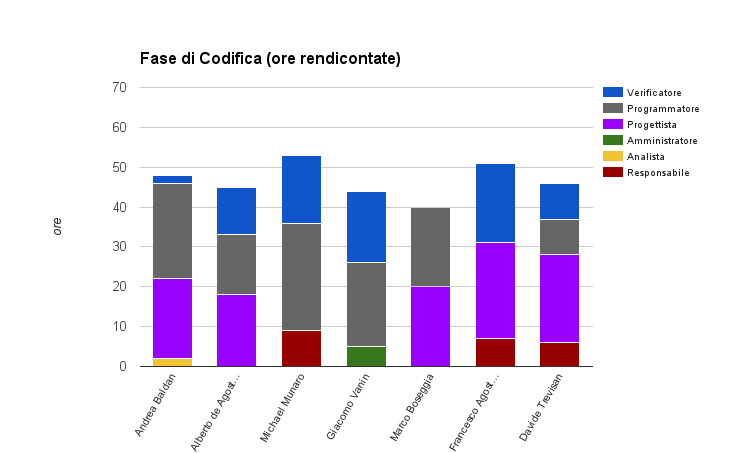
\includegraphics[width=1.2\textwidth,keepaspectratio]{CodificaConRendicontazione.png}
    \caption{Ore con rendicontazione, fase di Codifica}
  \end{subfigure}
\end{figure}
\newpage
\subsection{Prospetto economico}
In questa sottosezione vengono presentati, per ciascuna fase del progetto identificata
nella sottosezione \ref{sub:fasi}, le ore preventivate di impiego per i ruoli coinvolti.
\subsubsection{Analisi}
Nella fase di Analisi, le ore tra i ruoli sono state divise nel seguente modo:
\begin{center}
  \normalsize
  \begin{tabular}{| c | c | c |}
    \hline
    \multicolumn{3}{|c|}{\textbf{Con investimento}}\\
    \hline
    \textbf{Ruolo} & \textbf{Ore} & \textbf{Costo}\\
    \hline
    Responsabile & 27 & 810\\
    Amministratore & 23 & 460\\
    Analista & 97 & 2425\\
    Progettista & 0 & 0\\
    Verificatore & 114 & 1710 \\
    Programmatore & 0 & 0 \\
    \hline
    \textbf{Totale} & 261 & 5405\\
    \hline
  \end{tabular}
  \qquad
  \begin{tabular}{| c | c | c |}
    \hline
    \multicolumn{3}{|c|}{\textbf{Senza investimento}}\\
    \hline
    \textbf{Ruolo} & \textbf{Ore} & \textbf{Costo}\\
    \hline
    Responsabile & 25 & 750\\
    Amministratore & 18 & 360\\
    Analista & 85 & 2125\\
    Progettista & 0 & 0\\
    Verificatore & 98 & 1470 \\
    Programmatore & 0 & 0 \\
    \hline
    \textbf{Totale} & 226 & 4705\\
    \hline
  \end{tabular}
\end{center}
I grafici a seguire rappresentano l'influenza di ciascun ruolo sul totale delle ore e dei costi in fase di Analisi.
\begin{figure}[H]
  \begin{subfigure}[H]{0.47\textwidth}
    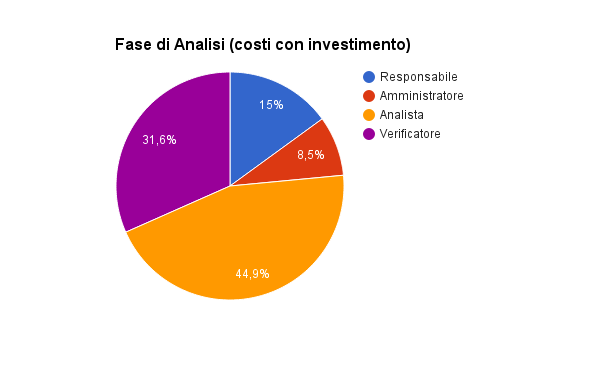
\includegraphics[width=1.2\textwidth,keepaspectratio]{AnalisiCC.png}
    \caption{Costi con investimento, fase di Analisi}
  \end{subfigure}
  \qquad
  \begin{subfigure}[H]{0.47\textwidth}
    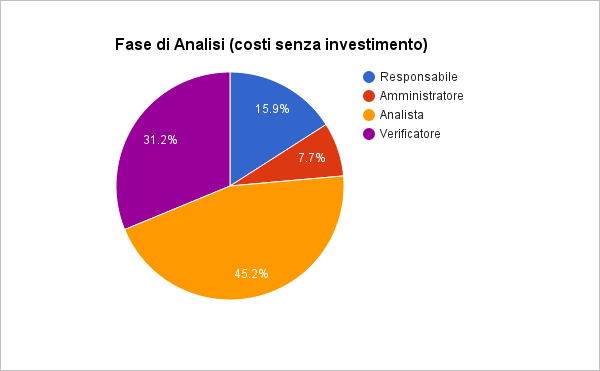
\includegraphics[width=1.2\textwidth,keepaspectratio]{AnalisiSC.png}
    \caption{Costi Senza investimento, fase di Analisi}
  \end{subfigure}
\end{figure}
\newpage
\subsubsection{Progettazione}
Nella fase di Progettazione, le ore tra i ruoli sono state divise nel seguente modo:
\begin{center}
  \normalsize
  \begin{tabular}{| c | c | c |}
    \hline
    \multicolumn{3}{|c|}{\textbf{Con investimento}}\\
    \hline
    \textbf{Ruolo} & \textbf{Ore} & \textbf{Costo}\\
    \hline
    Responsabile & 19 & 570\\
    Amministratore & 8 & 160\\
    Analista & 19 & 475\\
    Progettista & 94 & 2068\\
    Verificatore & 55 & 825 \\
    Programmatore & 0 & 0 \\
    \hline
    \textbf{Totale} & 195 & 4098\\
    \hline
  \end{tabular}
  \qquad
  \begin{tabular}{| c | c | c |}
    \hline
    \multicolumn{3}{|c|}{\textbf{Senza investimento}}\\
    \hline
    \textbf{Ruolo} & \textbf{Ore} & \textbf{Costo}\\
    \hline
    Responsabile & 16 & 480\\
    Amministratore & 7 & 140\\
    Analista & 16 & 400\\
    Progettista & 82 & 1804\\
    Verificatore & 43 & 645 \\
    Programmatore & 0 & 0 \\
    \hline
    \textbf{Totale} & 164 & 3469\\
    \hline
  \end{tabular}
\end{center}
I grafici a seguire rappresentano l'influenza di ciascun ruolo sul totale delle ore e dei costi in fase di Progettazione.
\begin{figure}[H]
  \begin{subfigure}[H]{0.47\textwidth}
    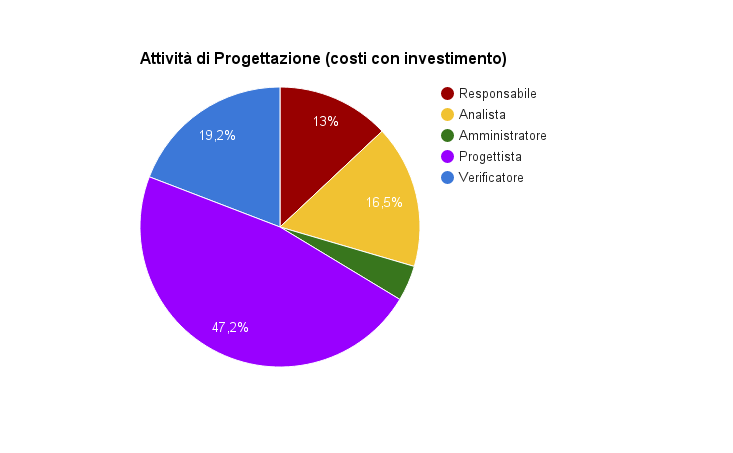
\includegraphics[width=1.2\textwidth,keepaspectratio]{ProgettazioneCC.png}
    \caption{Costi con investimento, fase di Progettazione}
  \end{subfigure}
  \qquad
  \begin{subfigure}[H]{0.47\textwidth}
    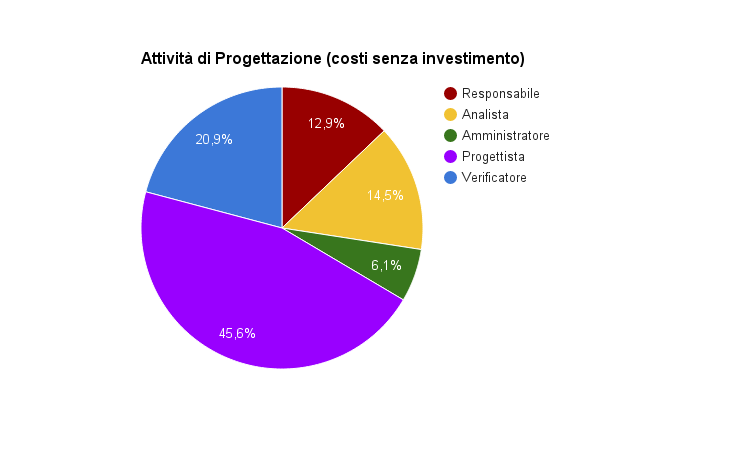
\includegraphics[width=1.2\textwidth,keepaspectratio]{ProgettazioneSC.png}
    \caption{Costi con investimento, fase di Progettazione}
  \end{subfigure}
\end{figure}
\newpage
\subsubsection{Codifica}
Nella fase di Codifica, le ore tra i ruoli sono state divise nel seguente modo:
\begin{center}
  \normalsize
  \begin{tabular}{| c | c | c |}
    \hline
    \multicolumn{3}{|c|}{\textbf{Con investimento}}\\
    \hline
    \textbf{Ruolo} & \textbf{Ore} & \textbf{Costo}\\
    \hline
    Responsabile & 24 & 720\\
    Amministratore & 6 & 120\\
    Analista & 2 & 50\\
    Progettista & 117 & 2574\\
    Verificatore & 102 & 1530 \\
    Programmatore & 130 & 1950 \\
    \hline
    \textbf{Totale} & 381 & 6944\\
    \hline
  \end{tabular}
  \qquad
  \begin{tabular}{| c | c | c |}
    \hline
    \multicolumn{3}{|c|}{\textbf{Senza investimento}}\\
    \hline
    \textbf{Ruolo} & \textbf{Ore} & \textbf{Costo}\\
    \hline
    Responsabile & 22 & 660\\
    Amministratore & 5 & 100\\
    Analista & 2 & 50\\
    Progettista & 104 & 2288\\
    Verificatore & 78 & 1170 \\
    Programmatore & 116 & 1740 \\
    \hline
    \textbf{Totale} & 327 & 6008 \\
    \hline
  \end{tabular}
\end{center}
I grafici a seguire rappresentano l'influenza di ciascun ruolo sul totale delle ore e dei costi in fase di Codifica 
\begin{figure}[H]
  \begin{subfigure}[H]{0.47\textwidth}
    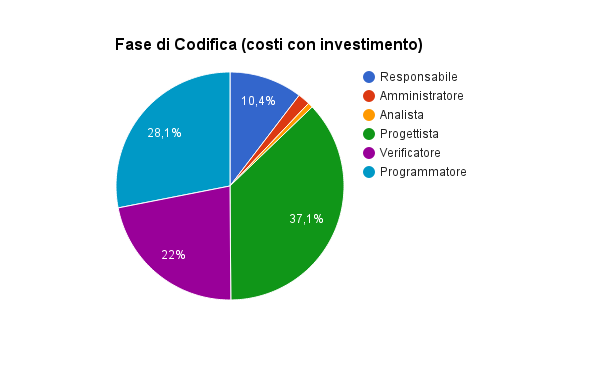
\includegraphics[width=1.2\textwidth,keepaspectratio]{CodificaCC.png}
    \caption{Costi con investimento, fase di Codifica}
  \end{subfigure}
  \qquad
  \begin{subfigure}[H]{0.47\textwidth}
    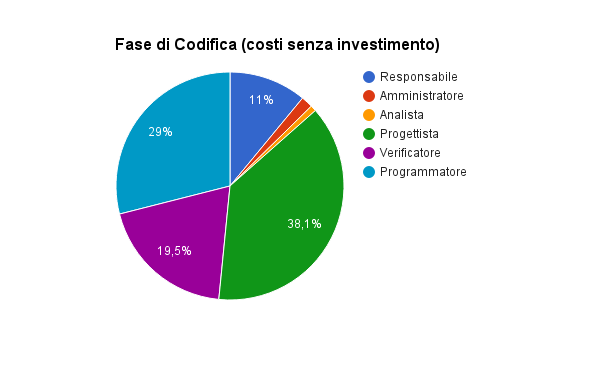
\includegraphics[width=1.2\textwidth,keepaspectratio]{CodificaSC.png}
    \caption{Costi senza investimento, fase di Codifica}
  \end{subfigure}
\end{figure}
\newpage
\subsection{Totale}
Le ore rendicontate totali, previste per la realizzazione del prodotto, senza
investimento sono:
\begin{center}
  \normalsize
  \begin{tabular}{| c | c | c |}
    \hline
    \multicolumn{3}{|c|}{\textbf{Con investimento}}\\
    \hline
    \textbf{Ruolo} & \textbf{Ore} & \textbf{Costo}\\
    \hline
    Responsabile & 70 & 2100\\
    Amministratore & 37 & 740\\
    Analista & 118 & 2950\\
    Progettista & 211 & 4642\\
    Verificatore & 271 & 4065 \\
    Programmatore & 130 & 1950 \\
    \hline
    \textbf{Totale} & 837 & 16447\\
    \hline
  \end{tabular}
  \qquad
  \begin{tabular}{| c | c | c |}
    \hline
    \multicolumn{2}{|c|}{\textbf{Senza investimento}}\\
    \hline
    \textbf{Ruolo} & \textbf{Ore} & \textbf{Costo}\\
    \hline
    Responsabile & 63 & 1890\\
    Amministratore & 30 & 600\\
    Analista & 103 & 2575\\
    Progettista & 186 & 4092\\
    Verificatore & 219 & 3285\\
    Programmatore & 116 & 1740 \\
    \hline
    \textbf{Totale} & 717 & 14182 \\
    \hline
  \end{tabular}
\end{center}
I grafici a seguire rappresentano l'influenza di ciascun ruolo sul totale delle ore e dei costi Complessivi.
\begin{figure}[H]
  \begin{subfigure}[H]{0.47\textwidth}
    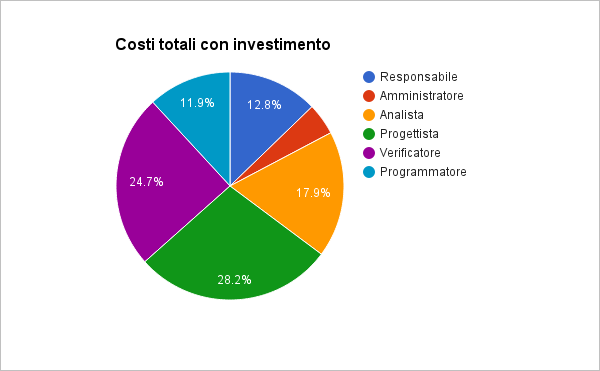
\includegraphics[width=1.0\textwidth,keepaspectratio]{TotaliCC.png}
    \caption{Costi con investimento, costi Totali}
  \end{subfigure}
  \qquad
  \begin{subfigure}[H]{0.47\textwidth}
    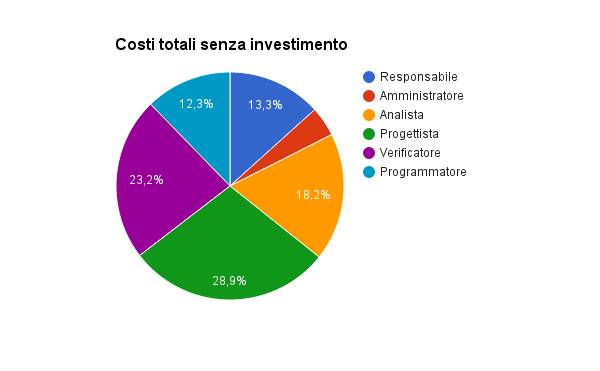
\includegraphics[width=1.0\textwidth,keepaspectratio]{TotaliSC.png}
    \caption{Costi senza investimento, costi Totali}
  \end{subfigure}
\end{figure}
\section{Analisi dei rischi}
L'analisi dei rischi ha costituito una fase critica della pianificazione, in
quanto l'azienda, alla sua prima esperienza, ha dovuto pensare agli ipotetici
scenari negativi che possono formarsi col procedere della fase di sviluppo.
\subsection{Identificazione del rischio}
Per l'identificazione dei rischi il primo passo è stato un' attività di
\gloss{Brainstorming} suddiviso per categorie di pertinenza, in modo da esplorare
in maniera quanto più generale e ampia possibile i vari aspetti di ogni
possibile scenario, seguito da una fase di analisi di ogni rischio emerso e
l'impatto che questo avrebbe portato al raggiungimento degli obiettivi preposti
per la conclusione del progetto. Le categorie prese in considerazione sono:
\begin{itemize}
\item\textbf{Logistica}
\item\textbf{Competenza tecnica}
\item\textbf{Infrastruttura}
\end{itemize}
\subsubsection{Parametri di quantificazione dei rischi}
Per ogni possibile rischio previsto l'analisi ha fornito i seguenti parametri:
\begin{itemize}
\item\textbf{Categoria}: Indica la categoria di appartenenza in cui ricade il
  rischio preso in considerazione
\item\textbf{Probabilità}: Probabilità statistica che lo scenario indesiderato
  si presenti, può assumere i seguenti valori:
  \begin{itemize}
  \item\textbf{Basso}
  \item\textbf{Medio}
  \item\textbf{Alto}
  \item\textbf{Molto alto}
  \end{itemize}
\item\textbf{Impatto}: Grado di pericolosità dello scenario indesiderato, può
  assumere i seguenti valori:
  \begin{itemize}
  \item\textbf{Molto Forte}
  \item\textbf{Forte}
  \item\textbf{Medio}
  \item\textbf{Debole}
  \end{itemize}
\item\textbf{Descrizione}: Una descrizione del caso preso in considerazione.
\item\textbf{Contromisure di mitigazione}: Provvedimenti da attuare in
  previsione del rischio, e/o di mitigazione in caso di bisogno
\end{itemize}
\begin{table}[H]
  \centering
  \scriptsize
  \caption{Tabella Analisi dei Rischi}
  \begin{tabular}{|m{1cm}|m{3cm}|m{3cm}|m{3cm}|m{3cm}|}
    \hline
    & \multicolumn{4}{|c|}{\textbf{Probabilità}}\\
    \hline
    \bf Impatto & \bf Bassa & \bf Media & \bf Alta & \textbf{Molto alta} \\
    \hline
    \bf Molto Forte & \cellcolor{red!50} & \cellcolor{red!50} & \cellcolor{red!50} &\cellcolor{red!50} \\
    \hline
    \bf Forte & \cellcolor{yellow!50}Guasti hardware & \cellcolor{yellow!50}Stime attività & \cellcolor{red!50}Analisi requisiti &\cellcolor{red!50}\\[8pt]
    \hline
    \bf Medio & \cellcolor{green!50} & \cellcolor{yellow!50} &\cellcolor{yellow!50}Tecnologia di impiego &\cellcolor{red!50}Inesperienza \\[8pt]
    \hline
    \bf Debole & \cellcolor{green!50}Dissensi tra componenti & \cellcolor{green!50} &\cellcolor{yellow!50}Ambiente di lavoro non omogeneo &\cellcolor{yellow!50}Impegni personali \\
    \hline
  \end{tabular} \\
\end{table}
\begin{table}[H]
  \centering
  \caption{Legenda colorazione rischi}
  \begin{tabular}{|c|c|l|}
    \hline \bf Colore & \bf Probabilità & \bf Legenda \\
    \hline \cellcolor{red! 50} & p > 75\% & Rischio non accettabile - riduzione obbligatoria \\
    \hline \cellcolor{yellow! 50} & 25\% < p < 75\% & Rischio accettabile. Considerare una riduzione. \\
    \hline \cellcolor{green! 50} & p < 25\% & Accettabile. \\
    \hline
  \end{tabular}
\end{table}
\paragraph{Impegni personali}
\textbf{Categoria}: Logistica\\
\textbf{Probabilità}: Alta\\
\textbf{Impatto}: Debole\\
\textbf{Descrizione}: Il gruppo può avere problemi a riunirsi fisicamente con la maggior parte dei membri presenti.
\textbf{Contromisure di mitigazione}: Il \textit{Responsabile di Progetto} ha stabilito una frequenza di incontri fissa,
l'azienda ha inoltre creato alcuni canali di comunicazione remota in modo da poter lavorare quanto più possibile in
coordinazione reciproca.
\paragraph{Inesperienza}
\textbf{Categoria}: Competenza tecnica\\
\textbf{Probabilità}: Alta\\
\textbf{Impatto}: Forte\\
\textbf{Descrizione}: Il gruppo può rimanere spiazzato dal metodo di lavoro da seguire, l'inesperienza nell'attuazione
di competenze di pianificazione e analisi può portare a rallentamenti del perseguimento degli obiettivi.
\textbf{Contromisure di mitigazione}: I componenti del gruppo si impegneranno a studiare e applicarsi il più possibile
nella pratica delle competenze richieste, ed eventualmente, il \textit{Responsabile} potrà riassegnare alcuni ruoli provvisoriamente
basandosi sui punti deboli e forti dei componenti con maggiore difficoltà a portare a termine la propria \gloss{attività}.
\paragraph{Tecnologia di impiego}
\textbf{Categoria}: Competenza tecnica\\
\textbf{Probabilità}: Alta\\
\textbf{Impatto}: Forte\\
\textbf{Descrizione}: Le tecnologie impiegate nello sviluppo del progetto poggiano su principi noti in buona misura a tutti
i componenti del gruppo, tuttavia l'assenza di un grado di specializzazione tangibile può generare lacune anche gravi nell' utilizzo
degli strumenti in questione.
\textbf{Contromisure di mitigazione}: Ciascun componente del gruppo avrà il compito di documentarsi costantemente e applicarsi
nell'uso delle tecnologie del progetto.
\paragraph{Ambiente di lavoro omogeneo}
\textbf{Categoria}: Infrastruttura\\
\textbf{Probabilità}: Alta\\
\textbf{Impatto}: Debole\\
\textbf{Descrizione}: La quantità di strumenti da utilizzare e la loro grande versatilità, oltre a renderli potenti, genera anche
la necessità di un ambiente di lavoro quanto più omogeneo possibile, in modo da semplificare lo sviluppo e avere un comportamento
da parte delle macchine il più comune possibile, in modo da garantire eventualmente anche la riproducibilità di bug che possono
insorgere.
\textbf{Contromisure di mitigazione}: L'azienda (\textit{Responsabile}?) ha deciso di risolvere il problema utilizzando una macchina virtuale
preimpostata per l'utilizzo delle tecnologie inerenti al progetto per la fase di sviluppo.
\paragraph{Guasti hardware}
\textbf{Categoria}: Infrastruttura\\
\textbf{Probabilità}: Bassa\\
\textbf{Impatto}: Forte\\
\textbf{Descrizione}: Buona parte del lavoro poggia su server privato gestito dall'\textit{Amministratore} su direttive dal \textit{Responsabile},
questo garantisce un buon grado di controllo, ma allo stesso tempo espone a maggiori rischi legati alla natura "personalizzata" dell'ambiente di lavoro.
\textbf{Contromisure di mitigazione}: Verranno eseguiti dei backup automatici schedulati con periodicità fissa.
\end{document}
